% ĐỢT 6: CỤM 4 (ĐỀ 2 & ĐỀ 3) - BỘ ĐỀ THAM KHẢO TUYỂN SINH 10 NĂM HỌC 2026-2027 SỞ GD&ĐT TP.HCM

% ==============================================================================
% CỤM 4 - ĐỀ THAM KHẢO 2 (Trang 23-24, Đề số 11)
% ==============================================================================

\begin{bt}%[9D6H18-2]
% nguon: Đề tham khảo Tuyển sinh 10 năm học 2026-2027 Sở GD&ĐT TP.HCM - Cụm 4 Đề 2 - Bài 1
Cho hàm số $y = \dfrac{x^2}{2}$ có đồ thị là Parabol $(P)$.
\begin{enumerate}[a)]
	\item Vẽ đồ thị $(P)$ trên mặt phẳng tọa độ $Oxy$.
	\item Tìm tọa độ các điểm thuộc $(P)$ có tung độ gấp đôi hoành độ.
\end{enumerate}
\loigiai{
\begin{enumerate}[a)]
	\item Bảng giá trị của hàm số $y = \dfrac{x^2}{2}$:
	\begin{center}
		\begin{tabular}{|c|c|c|c|c|c|}
			\hline
			$x$ & $-4$ & $-2$ & $0$ & $2$ & $4$ \\ \hline
			$y$ & $8$ & $2$ & $0$ & $2$ & $8$ \\ \hline
		\end{tabular}
	\end{center}
	Đồ thị $(P)$ là một đường parabol đi qua các điểm $(-4; 8)$, $(-2; 2)$, $(0; 0)$, $(2; 2)$, $(4; 8)$, nhận trục tung $Oy$ làm trục đối xứng và có đỉnh là gốc tọa độ $O(0;0)$.
	\begin{center}
		\begin{tikzpicture}[>=stealth,scale=0.7]
			\draw[->] (-5,0) -- (5,0) node[below] {$x$};
			\draw[->] (0,-1) -- (0,9) node[left] {$y$};
			\draw (0,0) node[below right] {$O$};
			\foreach \x in {-4,-2,2,4}
				\draw (\x,0.1) -- (\x,-0.1) node[below] {\small $\x$};
			\foreach \y in {2,8}
				\draw (0.1,\y) -- (-0.1,\y) node[left] {\small $\y$};
			\draw[dashed] (-2,0) -- (-2,2) -- (2,2) -- (2,0);
			\draw[dashed] (-4,0) -- (-4,8) -- (4,8) -- (4,0);
			\draw[thick,smooth,samples=100,domain=-4.1:4.1] plot(\x,{0.5*(\x)^2});
			\node[above left] at (2,2) {$(P)$};
		\end{tikzpicture}
	\end{center}
	\item Gọi điểm cần tìm là $M(x; y)$. Vì điểm $M$ thuộc $(P)$ và có tung độ gấp đôi hoành độ nên $y = 2x$.\\
	Ta có phương trình hoành độ giao điểm:
	$$\dfrac{x^2}{2} = 2x \iff \dfrac{x^2}{2} - 2x = 0 \iff x\left(\dfrac{x}{2} - 2\right) = 0 \iff \left[\begin{aligned} &x = 0 \\ &x = 4. \end{aligned}\right.$$
	\begin{itemize}
		\item Với $x = 0 \implies y = 0$, ta được điểm $O(0; 0)$.
		\item Với $x = 4 \implies y = 2 \cdot 4 = 8$, ta được điểm $A(4; 8)$.
	\end{itemize}
	Vậy tọa độ các điểm cần tìm là $(0; 0)$ và $(4; 8)$.
\end{enumerate}
}
\end{bt}

\begin{bt}%[9D6H20-2]
% nguon: Đề tham khảo Tuyển sinh 10 năm học 2026-2027 Sở GD&ĐT TP.HCM - Cụm 4 Đề 2 - Bài 2
Cho phương trình bậc hai $2025x^2 + 2025x - 2 = 0$.
\begin{enumerate}[a)]
	\item Chứng minh phương trình đã cho luôn có hai nghiệm phân biệt $x_1, x_2$.
	\item Không giải phương trình, hãy tính giá trị của biểu thức:
	$$T = \sqrt{\dfrac{(x_1 + x_2)^{2026}}{\dfrac{1}{4}(x_1 - x_2)^2 + \dfrac{2027}{8}x_1 x_2}}.$$
\end{enumerate}
\loigiai{
\begin{enumerate}[a)]
	\item Phương trình $2025x^2 + 2025x - 2 = 0$ có các hệ số $a = 2025$, $b = 2025$, $c = -2$.\\
	Biệt thức:
	$$\Delta = b^2 - 4ac = 2025^2 - 4 \cdot 2025 \cdot (-2) = 2025^2 + 16200 > 0.$$
	Vì $\Delta > 0$ nên phương trình luôn có hai nghiệm phân biệt $x_1, x_2$.
	\item Theo định lí Vi-ét, ta có:
	$$\left\{\begin{aligned} &x_1 + x_2 = -\dfrac{b}{a} = -\dfrac{2025}{2025} = -1 \\ &x_1 x_2 = \dfrac{c}{a} = -\dfrac{2}{2025}. \end{aligned}\right.$$
	Biến đổi biểu thức ở mẫu số trong dấu căn:
	\begin{align*}
		\dfrac{1}{4}(x_1 - x_2)^2 + \dfrac{2027}{8}x_1 x_2 &= \dfrac{1}{4}\left[(x_1 + x_2)^2 - 4x_1 x_2\right] + \dfrac{2027}{8}x_1 x_2 \\
		&= \dfrac{1}{4}(x_1 + x_2)^2 - x_1 x_2 + \dfrac{2027}{8}x_1 x_2 \\
		&= \dfrac{1}{4}(x_1 + x_2)^2 + \dfrac{2019}{8}x_1 x_2.
	\end{align*}
	Thay $x_1 + x_2 = -1$ và $x_1 x_2 = -\dfrac{2}{2025}$ vào mẫu số, ta được:
	$$\dfrac{1}{4}(-1)^2 + \dfrac{2019}{8} \cdot \left(-\dfrac{2}{2025}\right) = \dfrac{1}{4} - \dfrac{2019}{4 \cdot 2025} = \dfrac{2025 - 2019}{4 \cdot 2025} = \dfrac{6}{8100} = \dfrac{1}{1350}.$$
	Tử số là: $(x_1 + x_2)^{2026} = (-1)^{2026} = 1$.\\
	Do đó giá trị của biểu thức $T$ là:
	$$T = \sqrt{\dfrac{1}{\dfrac{1}{1350}}} = \sqrt{1350} = \sqrt{225 \cdot 6} = 15\sqrt{6}.$$
	Vậy $T = 15\sqrt{6}$.
\end{enumerate}
}
\end{bt}

\begin{bt}%[9D8H26-3]
% nguon: Đề tham khảo Tuyển sinh 10 năm học 2026-2027 Sở GD&ĐT TP.HCM - Cụm 4 Đề 2 - Bài 3
Số lượng huy chương Vàng, Bạc và Đồng của $10$ quốc gia tham dự SEA Games 33 được thống kê trong bảng sau:
\begin{center}
	\begin{tabular}{|l|c|c|c|c|c|c|c|c|c|c|}
		\hline
		\textbf{Loại huy chương} & \textbf{TL} & \textbf{INA} & \textbf{VN} & \textbf{MAS} & \textbf{SGP} & \textbf{PHI} & \textbf{MYA} & \textbf{LAO} & \textbf{BRU} & \textbf{TLS} \\ \hline
		\textbf{Huy chương Vàng} & $233$ & $91$ & $87$ & $57$ & $52$ & $50$ & $3$ & $2$ & $1$ & $0$ \\ \hline
		\textbf{Huy chương Bạc} & $154$ & $111$ & $81$ & $57$ & $61$ & $73$ & $21$ & $9$ & $3$ & $1$ \\ \hline
		\textbf{Huy chương Đồng} & $112$ & $131$ & $110$ & $117$ & $89$ & $154$ & $49$ & $28$ & $5$ & $7$ \\ \hline
	\end{tabular}
\end{center}
\begin{enumerate}[a)]
	\item Tỉ lệ phần trăm số huy chương Vàng của Việt Nam so với tổng số huy chương Vàng của $10$ quốc gia trong bảng là bao nhiêu? (Kết quả làm tròn đến hàng phần mười).
	\item Tính tổng số huy chương Vàng, Bạc, Đồng của mỗi quốc gia.
	\item Trong $10$ quốc gia ở bảng trên, chọn ngẫu nhiên $1$ quốc gia (mỗi quốc gia có khả năng được chọn như nhau). Tính xác suất để quốc gia được chọn có tổng số huy chương lớn hơn giá trị trung bình tổng số huy chương của cả $10$ quốc gia.
\end{enumerate}
\loigiai{
\begin{enumerate}[a)]
	\item Tổng số huy chương Vàng của cả $10$ quốc gia là:
	$$233 + 91 + 87 + 57 + 52 + 50 + 3 + 2 + 1 + 0 = 576\text{ (huy chương)}.$$
	Tỉ lệ phần trăm số huy chương Vàng của Việt Nam là:
	$$\dfrac{87}{576} \cdot 100\% \approx 15{,}1\%.$$
	\item Tổng số huy chương Vàng, Bạc, Đồng của từng quốc gia:
	\begin{itemize}
		\item Thái Lan: $233 + 154 + 112 = 499$ huy chương.
		\item Indonesia: $91 + 111 + 131 = 333$ huy chương.
		\item Việt Nam: $87 + 81 + 110 = 278$ huy chương.
		\item Malaysia: $57 + 57 + 117 = 231$ huy chương.
		\item Singapore: $52 + 61 + 89 = 202$ huy chương.
		\item Philippines: $50 + 73 + 154 = 277$ huy chương.
		\item Myanmar: $3 + 21 + 49 = 73$ huy chương.
		\item Lào: $2 + 9 + 28 = 39$ huy chương.
		\item Brunei: $1 + 3 + 5 = 9$ huy chương.
		\item Timor-Leste: $0 + 1 + 7 = 8$ huy chương.
	\end{itemize}
	\item Không gian mẫu là chọn ngẫu nhiên $1$ quốc gia trong $10$ quốc gia, nên $n(\Omega) = 10$.\\
	Tổng số huy chương của cả $10$ quốc gia là:
	$$499 + 333 + 278 + 231 + 202 + 277 + 73 + 39 + 9 + 8 = 1949\text{ (huy chương)}.$$
	Giá trị trung bình tổng số huy chương của $10$ quốc gia là:
	$$\bar{x} = \dfrac{1949}{10} = 194{,}9\text{ (huy chương)}.$$
	Gọi $A$ là biến cố: ``Quốc gia được chọn có tổng số huy chương lớn hơn $194{,}9$''.\\
	Các quốc gia có tổng số huy chương lớn hơn $194{,}9$ gồm $6$ quốc gia: Thái Lan ($499$), Indonesia ($333$), Việt Nam ($278$), Malaysia ($231$), Singapore ($202$), Philippines ($277$).\\
	Số kết quả thuận lợi cho biến cố $A$ là $n(A) = 6$.\\
	Xác suất của biến cố $A$ là:
	$$P(A) = \dfrac{n(A)}{n(\Omega)} = \dfrac{6}{10} = \dfrac{3}{5}.$$
\end{enumerate}
}
\end{bt}

\begin{bt}%[9D6V21-3]
% nguon: Đề tham khảo Tuyển sinh 10 năm học 2026-2027 Sở GD&ĐT TP.HCM - Cụm 4 Đề 2 - Bài 4
Một khu vườn hình chữ nhật có chiều dài $8a$ mét và chiều rộng $6a$ mét (với $a > 0$). Bác Hai xây một ao cá hình thoi, trong đó bốn đỉnh của hình thoi lần lượt là trung điểm các cạnh của khu vườn, phần đất còn lại bác trồng cỏ nhung.
\begin{enumerate}[a)]
	\item Tìm $a$ biết chu vi của ao cá hình thoi là $100$ mét.
	\item Biết chi phí trồng cỏ nhung là $65\,000$ đồng cho mỗi mét vuông. Tính số tiền (triệu đồng) bác Hai cần trả để trồng cỏ nhung.
\end{enumerate}
\loigiai{
\begin{enumerate}[a)]
	\item Gọi hình chữ nhật là $ABCD$, các trung điểm của các cạnh $AB, BC, CD, DA$ lần lượt là $M, N, P, Q$.\\
	Vì $M$ là trung điểm cạnh $AB$ nên $MB = \dfrac{8a}{2} = 4a\text{ (m)}$.\\
	Vì $N$ là trung điểm cạnh $BC$ nên $BN = \dfrac{6a}{2} = 3a\text{ (m)}$.\\
	Tam giác $MBN$ vuông tại $B$, áp dụng định lí Pythagore:
	$$MN = \sqrt{MB^2 + BN^2} = \sqrt{(4a)^2 + (3a)^2} = \sqrt{16a^2 + 9a^2} = \sqrt{25a^2} = 5a\text{ (m) (do } a > 0\text{)}.$$
	Chu vi của ao cá hình thoi $MNPQ$ là:
	$$4 \cdot MN = 4 \cdot 5a = 20a\text{ (m)}.$$
	Theo đề bài, chu vi của ao cá là $100\text{ m}$, ta có:
	$$20a = 100 \implies a = 5\text{ (m)}.$$
	\item Diện tích của khu vườn hình chữ nhật là:
	$$S_{\text{vườn}} = 8a \cdot 6a = 48a^2\text{ (m}^2\text{)}.$$
	Diện tích của ao cá hình thoi là:
	$$S_{\text{ao}} = \dfrac{1}{2} \cdot 8a \cdot 6a = 24a^2\text{ (m}^2\text{)}.$$
	Diện tích phần đất còn lại dùng để trồng cỏ nhung là:
	$$S_{\text{cỏ}} = S_{\text{vườn}} - S_{\text{ao}} = 48a^2 - 24a^2 = 24a^2\text{ (m}^2\text{)}.$$
	Với $a = 5\text{ m}$, diện tích trồng cỏ là:
	$$S_{\text{cỏ}} = 24 \cdot 5^2 = 600\text{ (m}^2\text{)}.$$
	Số tiền bác Hai cần trả để trồng cỏ nhung là:
	$$600 \cdot 65\,000 = 39\,000\,000\text{ (đồng)} = 39\text{ (triệu đồng)}.$$
	Vậy số tiền cần trả là $39$ triệu đồng.
\end{enumerate}
}
\end{bt}

\begin{bt}%[9H0V31-3]
% nguon: Đề tham khảo Tuyển sinh 10 năm học 2026-2027 Sở GD&ĐT TP.HCM - Cụm 4 Đề 2 - Bài 5
Một cái lon hình trụ có đường kính đáy $d = 2{,}9\text{ dm}$ chứa một lượng nước sao cho khi nhúng một quả cầu chạm đáy lon thì nước vừa ngập quả cầu. Biết rằng quả cầu không thấm nước và khi đặt vào vừa khít cái lon. Cho biết thể tích hình cầu là $V = \dfrac{4}{3}\pi R^3$ và thể tích hình trụ là $V = \pi r^2 h$.
\begin{enumerate}[a)]
	\item Tính thể tích của quả cầu theo đơn vị $\text{dm}^3$ (kết quả làm tròn đến hàng phần trăm).
	\item Tính chiều cao (theo đơn vị $\text{dm}$) của mực nước trong lon trước khi quả cầu được nhúng vào (làm tròn kết quả đến chữ số thập phân thứ hai).
\end{enumerate}
\loigiai{
\begin{enumerate}[a)]
	\item Bán kính của quả cầu là $R = \dfrac{d}{2} = \dfrac{2{,}9}{2} = 1{,}45\text{ (dm)}$.\\
	Thể tích của quả cầu là:
	$$V_{\text{cầu}} = \dfrac{4}{3}\pi R^3 = \dfrac{4}{3}\pi \cdot (1{,}45)^3 \approx \dfrac{4}{3} \cdot 3{,}14159 \cdot 3{,}048625 \approx 12{,}77\text{ (dm}^3\text{)}.$$
	\item Vì quả cầu đặt vừa khít vào lon hình trụ nên bán kính đáy lon bằng bán kính quả cầu: $r = R = 1{,}45\text{ dm}$.\\
	Khi thả quả cầu chạm đáy lon, nước vừa ngập quả cầu nên chiều cao mực nước lúc này bằng đường kính của quả cầu:
	$$h_{\text{sau}} = 2R = 2{,}9\text{ (dm)}.$$
	Thể tích của khối nước kết hợp với quả cầu tạo thành một khối trụ có chiều cao $h_{\text{sau}} = 2R$ và bán kính đáy $R$:\\
	Thể tích khối trụ đó là: $V_{\text{trụ}} = \pi R^2 \cdot (2R) = 2\pi R^3$.\\
	Thể tích của lượng nước ban đầu trong lon bằng:
	$$V_{\text{nước}} = V_{\text{trụ}} - V_{\text{cầu}} = 2\pi R^3 - \dfrac{4}{3}\pi R^3 = \dfrac{2}{3}\pi R^3.$$
	Gọi $h_0$ là chiều cao mực nước trong lon trước khi nhúng quả cầu vào. Ta có:
	$$V_{\text{nước}} = \pi R^2 h_0 \implies \pi R^2 h_0 = \dfrac{2}{3}\pi R^3 \implies h_0 = \dfrac{2}{3}R.$$
	Thay $R = 1{,}45\text{ dm}$, ta được:
	$$h_0 = \dfrac{2}{3} \cdot 1{,}45 = \dfrac{2{,}9}{3} \approx 0{,}97\text{ (dm)}.$$
	Vậy chiều cao của mực nước trong lon trước khi nhúng quả cầu là xấp xỉ $0{,}97\text{ dm}$.
\end{enumerate}
}
\end{bt}

\begin{bt}%[9D1H3-4]
% nguon: Đề tham khảo Tuyển sinh 10 năm học 2026-2027 Sở GD&ĐT TP.HCM - Cụm 4 Đề 2 - Bài 6
Hằng ngày, một chiếc thuyền đi xuôi dòng từ địa điểm $A$ đến địa điểm $B$ rồi quay trở về $A$ ngay sau đó. Một hôm, do công việc khẩn cấp nên vận tốc riêng của thuyền tăng lên gấp đôi thì thời gian đi từ $A$ đến $B$ rồi trở về $A$ ngay chỉ còn bằng $40\%$ so với thời gian thường lệ hằng ngày. Tính tỉ số giữa vận tốc riêng của thuyền trong mỗi chuyến đi ngày thường so với vận tốc của dòng nước (biết vận tốc của dòng nước không đổi và vận tốc riêng của thuyền là vận tốc của thuyền khi nước đứng yên).
\loigiai{
Gọi $v$ (km/h) là vận tốc riêng của thuyền trong ngày thường ($v > 0$).\\
Gọi $u$ (km/h) là vận tốc của dòng nước ($0 < u < v$).\\
Gọi $s$ (km) là độ dài quãng đường từ $A$ đến $B$ ($s > 0$).\\
Vào ngày thường:
\begin{itemize}
	\item Vận tốc xuôi dòng là $v + u$, thời gian xuôi dòng là $t_1 = \dfrac{s}{v + u}$.
	\item Vận tốc ngược dòng là $v - u$, thời gian ngược dòng là $t_2 = \dfrac{s}{v - u}$.
	\item Tổng thời gian cả đi lẫn về hằng ngày là:
	$$T = t_1 + t_2 = \dfrac{s}{v + u} + \dfrac{s}{v - u} = \dfrac{s(v - u + v + u)}{v^2 - u^2} = \dfrac{2sv}{v^2 - u^2}.$$
\end{itemize}
Vào hôm có công việc khẩn cấp:
\begin{itemize}
	\item Vận tốc riêng của thuyền tăng gấp đôi là $2v$.
	\item Vận tốc xuôi dòng là $2v + u$, thời gian xuôi dòng là $t'_1 = \dfrac{s}{2v + u}$.
	\item Vận tốc ngược dòng là $2v - u$, thời gian ngược dòng là $t'_2 = \dfrac{s}{2v - u}$.
	\item Tổng thời gian cả đi lẫn về hôm khẩn cấp là:
	$$T' = t'_1 + t'_2 = \dfrac{s}{2v + u} + \dfrac{s}{2v - u} = \dfrac{s(2v - u + 2v + u)}{4v^2 - u^2} = \dfrac{4sv}{4v^2 - u^2}.$$
\end{itemize}
Theo đề bài, thời gian $T'$ chỉ bằng $40\%$ thời gian $T$, tức là $T' = \dfrac{2}{5}T$. Do đó ta có phương trình:
$$\dfrac{4sv}{4v^2 - u^2} = \dfrac{2}{5} \cdot \dfrac{2sv}{v^2 - u^2}.$$
Vì $s > 0$ và $v > 0$, ta chia cả hai vế cho $4sv$:
$$\dfrac{1}{4v^2 - u^2} = \dfrac{1}{5(v^2 - u^2)} \iff 5(v^2 - u^2) = 4v^2 - u^2 \iff 5v^2 - 5u^2 = 4v^2 - u^2 \iff v^2 = 4u^2.$$
Vì $v > 0$ và $u > 0$ nên:
$$v = 2u \implies \dfrac{v}{u} = 2.$$
Vậy tỉ số giữa vận tốc riêng của thuyền ngày thường so với vận tốc dòng nước là $2$ (vận tốc riêng gấp $2$ lần vận tốc dòng nước).
}
\end{bt}

\begin{bt}%[9H9C29-3]
% nguon: Đề tham khảo Tuyển sinh 10 năm học 2026-2027 Sở GD&ĐT TP.HCM - Cụm 4 Đề 2 - Bài 7
Từ một điểm $A$ nằm ngoài đường tròn $(O; R)$, kẻ hai tiếp tuyến $AB, AC$ với đường tròn ($B, C$ là hai tiếp điểm). Vẽ đường kính $BS$ của đường tròn $(O)$. Đoạn thẳng $OA$ cắt đường tròn $(O)$ tại điểm $I$.
\begin{enumerate}[a)]
	\item Chứng minh $OA \perp BC$ tại $H$ và $BC^2 = 2 \cdot SC \cdot HA$.
	\item Gọi $r$ là bán kính đường tròn nội tiếp tam giác $ABC$. Tính độ dài đoạn thẳng $CS$ theo $R$ và $r$.
	\item Vẽ $HD \perp AB$ tại $D$. Lấy $F$ là trung điểm của đoạn thẳng $OB$, gọi $E$ là giao điểm của $AF$ với $CD$. Chứng minh bốn điểm $C, H, E, A$ cùng thuộc một đường tròn.
\end{enumerate}
\loigiai{
\begin{center}
	\begin{tikzpicture}[scale=0.9,>=stealth]
		\coordinate (O) at (0,0);
		\def\R{2.8}
		\draw[thick] (O) circle (\R);
		\coordinate (B) at (0,\R);
		\coordinate (S) at (0,-\R);
		% Tiep tuyen tai B la duong ngang y = R
		% Cho A nam ben trai: A(-4, R)
		\coordinate (A) at (-4,\R);
		% Tiep tuyen AC: C nam tren (O). goc AOB vuong tai B
		% OA vuong goc BC tai H
		% De ve AC: C la doi xung cua B qua OA
		\coordinate (H) at ($(A)!(O)!(B)$); % tam
		% Do AB la tiep tuyen tai B nen goc ABO = 90. A(-4, R), B(0, R), O(0,0) => ABO vuong tai B.
		\coordinate (M) at ($(A)!0.5!(O)$);
		\path [name path=circle] (O) circle (\R);
		\coordinate (C) at (-2.15,-1.79);
		\coordinate (H) at ($(B)!0.5!(C)$);
		\coordinate (I) at ($(O)!{\R/sqrt(16+\R*\R)}!(A)$);
		\coordinate (D) at ($(A)!(H)!(B)$);
		\coordinate (F) at ($(O)!0.5!(B)$);
		\coordinate (E) at (intersection of A--F and C--D);

		\draw[thick] (A) -- (B) -- (S);
		\draw[thick] (A) -- (C);
		\draw[thick] (B) -- (C) -- (S);
		\draw[thick] (O) -- (A);
		\draw[thick] (H) -- (D);
		\draw[thick] (A) -- (E);
		\draw[thick] (C) -- (E);
		\draw[dashed] (O) -- (C);

		\fill (O) circle (1.5pt) node[right] {$O$};
		\fill (B) circle (1.5pt) node[above] {$B$};
		\fill (S) circle (1.5pt) node[below] {$S$};
		\fill (A) circle (1.5pt) node[left] {$A$};
		\fill (C) circle (1.5pt) node[below left] {$C$};
		\fill (H) circle (1.5pt) node[above left] {$H$};
		\fill (I) circle (1.5pt) node[above right] {$I$};
		\fill (D) circle (1.5pt) node[above] {$D$};
		\fill (F) circle (1.5pt) node[right] {$F$};
		\fill (E) circle (1.5pt) node[left] {$E$};
	\end{tikzpicture}
\end{center}
\begin{enumerate}[a)]
	\item Ta có $AB = AC$ (tính chất hai tiếp tuyến cắt nhau) và $OB = OC = R$ (bán kính của $(O)$).\\
	Suy ra $OA$ là đường trung trực của đoạn thẳng $BC$, do đó $OA \perp BC$ tại $H$ và $H$ là trung điểm của $BC$.\\
	Xét tam giác $SBC$ có $O$ là trung điểm của $SB$ và $H$ là trung điểm của $BC$, nên $OH$ là đường trung bình của tam giác $SBC$.\\
	Suy ra $SC = 2 \cdot OH$.\\
	Xét tam giác $ABO$ vuông tại $B$ có đường cao $BH$ ($BH \perp OA$ tại $H$), áp dụng hệ thức lượng ta có:
	$$BH^2 = AH \cdot OH.$$
	Vì $H$ là trung điểm của $BC$ nên $BC = 2 \cdot BH \implies BC^2 = 4 \cdot BH^2$.\\
	Do đó:
	$$BC^2 = 4 \cdot AH \cdot OH = 2 \cdot HA \cdot (2 \cdot OH) = 2 \cdot SC \cdot HA.$$
	\item Tam giác $OCI$ có $OC = OI = R$ nên tam giác $OCI$ cân tại $O$, suy ra $\widehat{OCI} = \widehat{OIC}$.\\
	Vì $AC$ là tiếp tuyến của $(O)$ tại $C$ nên $AC \perp OC \implies \widehat{ACI} = 90^\circ - \widehat{OCI}$.\\
	Trong tam giác $HIC$ vuông tại $H$, ta có $\widehat{HCI} = 90^\circ - \widehat{HIC}$.\\
	Mà $\widehat{OCI} = \widehat{OIC} = \widehat{HIC}$, do đó $\widehat{ACI} = \widehat{HCI}$, tức là $CI$ là tia phân giác của góc $\widehat{ACB}$.\\
	Mặt khác, $AI$ là tia phân giác của góc $\widehat{BAC}$ (tính chất hai tiếp tuyến cắt nhau).\\
	Do đó $I$ là giao điểm các đường phân giác trong tam giác $ABC$, tức $I$ là tâm đường tròn nội tiếp tam giác $ABC$.\\
	Vì $IH \perp BC$ nên $IH = r$ (bán kính đường tròn nội tiếp $\Delta ABC$).\\
	Độ dài đoạn thẳng $OH$ là:
	$$OH = OI - IH = R - r.$$
	Vì $SC = 2 \cdot OH$ nên:
	$$CS = 2(R - r).$$
	\item Kẻ $CK \perp AB$ tại $K$. Vì $HD \perp AB$ nên $HD \parallel CK$.\\
	Xét tam giác $BCK$ có $H$ là trung điểm $BC$ và $HD \parallel CK$ nên $D$ là trung điểm của đoạn thẳng $BK$.\\
	Ta có $\widehat{AOB} = \widehat{CBK}$ (vì cùng phụ với góc $\widehat{OBH}$).\\
	Xét hai tam giác vuông $\Delta ABO$ và $\Delta CKB$ có:
	$$\widehat{ABO} = \widehat{CKB} = 90^\circ, \quad \widehat{AOB} = \widehat{CBK}.$$
	Do đó $\Delta ABO \backsim \Delta CKB$ (g-g) $\implies \dfrac{AB}{CK} = \dfrac{BO}{KB}$.\\
	Vì $F$ là trung điểm $OB \implies BO = 2BF$ và $D$ là trung điểm $BK \implies KB = 2KD$, nên:
	$$\dfrac{AB}{CK} = \dfrac{2BF}{2KD} = \dfrac{BF}{KD} \implies \dfrac{AB}{BF} = \dfrac{CK}{KD}.$$
	Xét $\Delta ABF$ và $\Delta CKD$ có:
	$$\widehat{ABF} = \widehat{CKD} = 90^\circ, \quad \dfrac{AB}{BF} = \dfrac{CK}{KD}.$$
	Do đó $\Delta ABF \backsim \Delta CKD$ (c-g-c) $\implies \widehat{BFA} = \widehat{CDK}$.\\
	Trong tam giác vuông $ABF$ vuông tại $B$, ta có $\widehat{BFA} + \widehat{BAF} = 90^\circ$.\\
	Suy ra $\widehat{CDK} + \widehat{BAF} = 90^\circ$, điều này chứng tỏ trong tam giác $ADE$, góc $\widehat{AED} = 90^\circ$ hay $AF \perp CD$ tại $E$.\\
	Tam giác $AEC$ vuông tại $E$ nên nội tiếp đường tròn đường kính $AC$.\\
	Tam giác $AHC$ vuông tại $H$ nên nội tiếp đường tròn đường kính $AC$.\\
	Vậy bốn điểm $C, H, E, A$ cùng thuộc một đường tròn (đường tròn đường kính $AC$).
\end{enumerate}
}
\end{bt}


% ==============================================================================
% CỤM 4 - ĐỀ THAM KHẢO 3 (Trang 25-26, Đề số 12)
% ==============================================================================

\begin{bt}%[9D6H18-2]
% nguon: Đề tham khảo Tuyển sinh 10 năm học 2026-2027 Sở GD&ĐT TP.HCM - Cụm 4 Đề 3 - Bài 1
Cho hàm số $y = -\dfrac{x^2}{4}$ có đồ thị là Parabol $(P)$.
\begin{enumerate}[a)]
	\item Vẽ đồ thị $(P)$ của hàm số trên mặt phẳng tọa độ $Oxy$.
	\item Tìm tọa độ các điểm $M$ thuộc đồ thị $(P)$ có tung độ bằng $2$ lần hoành độ.
\end{enumerate}
\loigiai{
\begin{enumerate}[a)]
	\item Bảng giá trị của hàm số $y = -\dfrac{x^2}{4}$:
	\begin{center}
		\begin{tabular}{|c|c|c|c|c|c|}
			\hline
			$x$ & $-4$ & $-2$ & $0$ & $2$ & $4$ \\ \hline
			$y$ & $-4$ & $-1$ & $0$ & $-1$ & $-4$ \\ \hline
		\end{tabular}
	\end{center}
	Đồ thị $(P)$ là một parabol đi qua các điểm $(-4; -4)$, $(-2; -1)$, $(0; 0)$, $(2; -1)$, $(4; -4)$, có đỉnh là gốc tọa độ $O(0;0)$ và nhận trục tung $Oy$ làm trục đối xứng.
	\begin{center}
		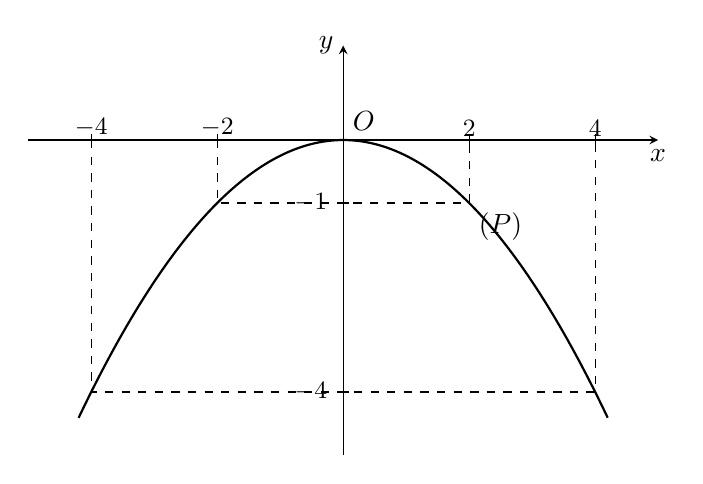
\begin{tikzpicture}[>=stealth,scale=0.8]
			\draw[->] (-5,0) -- (5,0) node[below] {$x$};
			\draw[->] (0,-5) -- (0,1.5) node[left] {$y$};
			\draw (0,0) node[above right] {$O$};
			\foreach \x in {-4,-2,2,4}
				\draw (\x,0.1) -- (\x,-0.1) node[above] {\small $\x$};
			\foreach \y in {-4,-1}
				\draw (0.1,\y) -- (-0.1,\y) node[left] {\small $\y$};
			\draw[dashed] (-2,0) -- (-2,-1) -- (2,-1) -- (2,0);
			\draw[dashed] (-4,0) -- (-4,-4) -- (4,-4) -- (4,0);
			\draw[thick,smooth,samples=100,domain=-4.2:4.2] plot(\x,{-0.25*(\x)^2});
			\node[below right] at (2,-1) {$(P)$};
		\end{tikzpicture}
	\end{center}
	\item Vì điểm $M$ thuộc $(P)$ có tung độ bằng $2$ lần hoành độ nên ta có $y = 2x$.\\
	Phương trình hoành độ giao điểm là:
	$$2x = -\dfrac{x^2}{4} \iff \dfrac{x^2}{4} + 2x = 0 \iff x\left(\dfrac{x}{4} + 2\right) = 0 \iff \left[\begin{aligned} &x = 0 \\ &x = -8. \end{aligned}\right.$$
	\begin{itemize}
		\item Với $x = 0 \implies y = 0$, ta được điểm $O(0; 0)$.
		\item Với $x = -8 \implies y = 2 \cdot (-8) = -16$, ta được điểm $M(-8; -16)$.
	\end{itemize}
	Vậy tọa độ các điểm cần tìm là $(0; 0)$ và $(-8; -16)$.
\end{enumerate}
}
\end{bt}

\begin{bt}%[9D6H20-2]
% nguon: Đề tham khảo Tuyển sinh 10 năm học 2026-2027 Sở GD&ĐT TP.HCM - Cụm 4 Đề 3 - Bài 2
Cho phương trình bậc hai $\sqrt{3}x^2 - 2x - \sqrt{3} = 0$.
\begin{enumerate}[a)]
	\item Chứng minh phương trình trên luôn có hai nghiệm phân biệt $x_1, x_2$.
	\item Không giải phương trình, hãy tính giá trị của biểu thức:
	$$C = 2\sqrt{3}x_1 - x_1^2 - x_2^2 - \sqrt{3}(x_1 - x_2).$$
\end{enumerate}
\loigiai{
\begin{enumerate}[a)]
	\item Phương trình $\sqrt{3}x^2 - 2x - \sqrt{3} = 0$ có các hệ số $a = \sqrt{3}$, $b = -2$, $c = -\sqrt{3}$.\\
	Ta có $a \cdot c = \sqrt{3} \cdot (-\sqrt{3}) = -3 < 0$.\\
	Vì $a$ và $c$ trái dấu nên phương trình luôn có hai nghiệm phân biệt $x_1, x_2$.
	\item Theo định lí Vi-ét, ta có:
	$$\left\{\begin{aligned} &x_1 + x_2 = -\dfrac{b}{a} = \dfrac{2}{\sqrt{3}} \\ &x_1 x_2 = \dfrac{c}{a} = \dfrac{-\sqrt{3}}{\sqrt{3}} = -1. \end{aligned}\right.$$
	Ta có:
	$$x_1^2 + x_2^2 = (x_1 + x_2)^2 - 2x_1 x_2 = \left(\dfrac{2}{\sqrt{3}}\right)^2 - 2(-1) = \dfrac{4}{3} + 2 = \dfrac{10}{3}.$$
	Biến đổi biểu thức $C$:
	\begin{align*}
		C &= 2\sqrt{3}x_1 - x_1^2 - x_2^2 - \sqrt{3}x_1 + \sqrt{3}x_2 \\
		&= \sqrt{3}x_1 + \sqrt{3}x_2 - (x_1^2 + x_2^2) \\
		&= \sqrt{3}(x_1 + x_2) - (x_1^2 + x_2^2).
	\end{align*}
	Thay các giá trị vào biểu thức $C$, ta được:
	$$C = \sqrt{3} \cdot \dfrac{2}{\sqrt{3}} - \dfrac{10}{3} = 2 - \dfrac{10}{3} = -\dfrac{4}{3}.$$
	Vậy $C = -\dfrac{4}{3}$.
\end{enumerate}
}
\end{bt}

\begin{bt}%[9D8H26-3]
% nguon: Đề tham khảo Tuyển sinh 10 năm học 2026-2027 Sở GD&ĐT TP.HCM - Cụm 4 Đề 3 - Bài 3
Biểu đồ cột kép sau đây biểu diễn số học sinh nam và số học sinh nữ của lớp 9A có sở thích chơi một số môn thể thao: bóng đá, bóng rổ, bơi:
\begin{center}
	\begin{tabular}{|l|c|c|c|}
		\hline
		\textbf{Môn thể thao} & \textbf{Bóng đá} & \textbf{Bóng rổ} & \textbf{Bơi} \\ \hline
		\textbf{Số học sinh nam} & $12$ & $4$ & $5$ \\ \hline
		\textbf{Số học sinh nữ} & $10$ & $5$ & $6$ \\ \hline
	\end{tabular}
\end{center}
\begin{enumerate}[a)]
	\item Tính số học sinh của lớp 9A (biết mỗi học sinh chỉ chọn đúng một môn thể thao yêu thích).
	\item Chọn ngẫu nhiên một học sinh của lớp 9A. Tính xác suất của biến cố: ``Học sinh được chọn là nữ và không thích bơi''.
\end{enumerate}
\loigiai{
\begin{enumerate}[a)]
	\item Tổng số học sinh nam của lớp 9A là:
	$$12 + 4 + 5 = 21\text{ (học sinh)}.$$
	Tổng số học sinh nữ của lớp 9A là:
	$$10 + 5 + 6 = 21\text{ (học sinh)}.$$
	Số học sinh của lớp 9A là:
	$$21 + 21 = 42\text{ (học sinh)}.$$
	\item Không gian mẫu là chọn ngẫu nhiên $1$ học sinh trong số $42$ học sinh của lớp, nên $n(\Omega) = 42$.\\
	Gọi $B$ là biến cố: ``Học sinh được chọn là nữ và không thích bơi''.\\
	Số học sinh nữ không thích bơi gồm các bạn nữ thích bóng đá và bóng rổ:
	$$n(B) = 10 + 5 = 15\text{ (học sinh)}.$$
	Xác suất của biến cố $B$ là:
	$$P(B) = \dfrac{n(B)}{n(\Omega)} = \dfrac{15}{42} = \dfrac{5}{14}.$$
\end{enumerate}
}
\end{bt}

\begin{bt}%[9D6V21-3]
% nguon: Đề tham khảo Tuyển sinh 10 năm học 2026-2027 Sở GD&ĐT TP.HCM - Cụm 4 Đề 3 - Bài 4
Nhóm bạn Tường Nguyên phác thảo một mô hình khu vườn hình chữ nhật có chiều dài $3\text{ m}$ và chiều rộng $2\text{ m}$. Nhóm lắp đặt hệ thống phun sương gồm: một phần chạy dọc theo chiều dài khu vườn, một phần nằm chính giữa khu vườn đều có độ rộng $x$ mét ($0 < x < 1$), và phần cuối mép dưới thiết kế dạng hình thang cân (đáy lớn $2\text{ m}$, đáy nhỏ $x\text{ m}$, chiều cao $x\text{ m}$). Phần diện tích còn lại dùng để trồng rau thủy canh.
\begin{enumerate}[a)]
	\item Hãy biểu diễn diện tích của phần hệ thống phun sương theo $x$.
	\item Nếu $x = 0{,}6$ thì diện tích phần đất trồng rau thủy canh là bao nhiêu mét vuông?
\end{enumerate}
\loigiai{
\begin{enumerate}[a)]
	\item Diện tích các phần cấu thành hệ thống phun sương:
	\begin{itemize}
		\item Phần chạy dọc theo chiều dài khu vườn (kích thước $3\text{ m} \times x\text{ m}$) có diện tích là $3x\text{ (m}^2\text{)}$.
		\item Phần hình thang cân (đáy lớn $2\text{ m}$, đáy nhỏ $x\text{ m}$, chiều cao $x\text{ m}$) có diện tích là:
		$$S_1 = \dfrac{(2 + x) \cdot x}{2} = x + 0{,}5x^2\text{ (m}^2\text{)}.$$
		\item Chiều cao của phần dải phun sương nằm ở chính giữa khu vườn là:
		$$2 - x - x = 2 - 2x\text{ (m)}.$$
		Diện tích của phần nằm giữa (kích thước $x \times (2 - 2x)$) là:
		$$S_2 = x(2 - 2x) = 2x - 2x^2\text{ (m}^2\text{)}.$$
	\end{itemize}
	Tổng diện tích của hệ thống phun sương là:
	$$S_{\text{HT}} = 3x + (x + 0{,}5x^2) + (2x - 2x^2) = -1{,}5x^2 + 6x\text{ (m}^2\text{)}.$$
	\item Diện tích của toàn bộ khu vườn là:
	$$S_{\text{vườn}} = 3 \cdot 2 = 6\text{ (m}^2\text{)}.$$
	Diện tích phần dùng để trồng rau thủy canh là:
	$$S_{\text{rau}} = S_{\text{vườn}} - S_{\text{HT}} = 6 - (-1{,}5x^2 + 6x) = 1{,}5x^2 - 6x + 6\text{ (m}^2\text{)}.$$
	Khi $x = 0{,}6$, diện tích phần trồng rau là:
	$$S_{\text{rau}} = 1{,}5 \cdot (0{,}6)^2 - 6 \cdot 0{,}6 + 6 = 1{,}5 \cdot 0{,}36 - 3{,}6 + 6 = 0{,}54 - 3{,}6 + 6 = 2{,}94\text{ (m}^2\text{)}.$$
	Vậy khi $x = 0{,}6$ thì diện tích phần trồng rau thủy canh là $2{,}94\text{ m}^2$.
\end{enumerate}
}
\end{bt}

\begin{bt}%[9H0V31-3]
% nguon: Đề tham khảo Tuyển sinh 10 năm học 2026-2027 Sở GD&ĐT TP.HCM - Cụm 4 Đề 3 - Bài 5
Một bồn nước hình trụ có đường kính đáy là $1{,}6\text{ m}$ và chiều cao là $2{,}3\text{ m}$. Lấy $\pi \approx 3{,}14$.
\begin{enumerate}[a)]
	\item Tính thể tích của bồn nước hình trụ đó.
	\item Người ta gắn một phao điện tự động vào nắp bồn nước. Khi lượng nước trong bồn chỉ còn $20\%$ dung tích của bồn thì máy bơm tự động bật để bơm nước vào. Khi mực nước dâng lên đến vị trí còn cách nắp bồn $10\text{ cm}$ thì máy bơm tự động ngắt điện. Biết công suất của máy bơm là $1086$ lít/giờ. Hỏi thời gian từ lúc máy bơm tự bật đến lúc máy bơm ngắt điện là bao nhiêu phút? (Làm tròn kết quả đến hàng đơn vị).
\end{enumerate}
\loigiai{
\begin{enumerate}[a)]
	\item Bán kính đáy của bồn nước hình trụ là $r = \dfrac{1{,}6}{2} = 0{,}8\text{ (m)}$.\\
	Thể tích của bồn nước hình trụ là:
	$$V = \pi r^2 h \approx 3{,}14 \cdot (0{,}8)^2 \cdot 2{,}3 = 4{,}62208\text{ (m}^3\text{)}.$$
	\item Đổi $10\text{ cm} = 0{,}1\text{ m}$.\\
	Thể tích nước còn lại trong bồn khi máy bơm bắt đầu bật là:
	$$V_1 = 20\% \cdot V = 0{,}2 \cdot 4{,}62208 = 0{,}924416\text{ (m}^3\text{)}.$$
	Chiều cao mực nước khi máy bơm tự động ngắt điện là:
	$$h_2 = 2{,}3 - 0{,}1 = 2{,}2\text{ (m)}.$$
	Thể tích nước trong bồn khi ngắt máy bơm là:
	$$V_2 = \pi r^2 h_2 \approx 3{,}14 \cdot (0{,}8)^2 \cdot 2{,}2 = 4{,}42112\text{ (m}^3\text{)}.$$
	Lượng nước cần bơm thêm vào bồn là:
	$$V_{\text{bơm}} = V_2 - V_1 = 4{,}42112 - 0{,}924416 = 3{,}496704\text{ (m}^3\text{)}.$$
	Đổi ra đơn vị lít ($1\text{ m}^3 = 1000\text{ lít}$):
	$$V_{\text{bơm}} = 3496{,}704\text{ (lít)}.$$
	Thời gian cần thiết để máy bơm bơm đủ lượng nước đó là:
	$$t = \dfrac{3496{,}704}{1086}\text{ (giờ)} = \dfrac{3496{,}704}{1086} \cdot 60 \approx 193{,}19\text{ (phút)}.$$
	Làm tròn đến hàng đơn vị là $193$ phút.\\
	Vậy thời gian từ khi máy bơm bật đến khi ngắt điện là khoảng $193$ phút.
\end{enumerate}
}
\end{bt}

\begin{bt}%[9D1H3-4]
% nguon: Đề tham khảo Tuyển sinh 10 năm học 2026-2027 Sở GD&ĐT TP.HCM - Cụm 4 Đề 3 - Bài 6
Trọng và Quốc chạy bộ trong khuôn viên có dạng hình tam giác vuông cân tại $A$ với $AB = AC = a\text{ (m)}$. Từ đỉnh $A$, hai bạn cùng lúc bắt đầu chạy bộ dọc theo các cạnh của tam giác với vận tốc không đổi nhưng theo hai chiều ngược nhau:
\begin{itemize}
	\item Trọng chạy theo chiều: $A \to B \to C \to A$.
	\item Quốc chạy theo chiều: $A \to C \to B \to A$.
\end{itemize}
Biết rằng lần gặp nhau thứ nhất, hai bạn gặp nhau tại điểm $M$ trên cạnh $BC$ với $BM = 600\text{ m}$. Sau đó, hai bạn tiếp tục chạy và gặp nhau lần thứ hai tại điểm $N$ trên cạnh $AB$ với $AN = 200\text{ m}$. Gọi $x, y$ (km/h) lần lượt là vận tốc chạy của Trọng và Quốc.
\begin{enumerate}[a)]
	\item Chứng minh rằng $\dfrac{x}{y} = \dfrac{AB + BM}{AC + CM}$.
	\item Tính độ dài các cạnh của khuôn viên tam giác đó (kết quả làm tròn đến hàng đơn vị).
\end{enumerate}
\loigiai{
\begin{enumerate}[a)]
	\item Gọi $t_1$ (giờ) là thời gian từ lúc xuất phát cho đến khi hai bạn gặp nhau lần thứ nhất tại $M$.\\
	Quãng đường Trọng chạy được trong thời gian $t_1$ là: $S_T = AB + BM$.\\
	Quãng đường Quốc chạy được trong thời gian $t_1$ là: $S_Q = AC + CM$.\\
	Vì vận tốc $x$ và $y$ của hai bạn không đổi nên ta có:
	$$x = \dfrac{S_T}{t_1} = \dfrac{AB + BM}{t_1}, \quad y = \dfrac{S_Q}{t_1} = \dfrac{AC + CM}{t_1}.$$
	Suy ra:
	$$\dfrac{x}{y} = \dfrac{x \cdot t_1}{y \cdot t_1} = \dfrac{AB + BM}{AC + CM}.$$
	\item Tam giác $ABC$ vuông cân tại $A$ có $AB = AC = a$ ($a > 200$), suy ra độ dài cạnh huyền là:
	$$BC = \sqrt{a^2 + a^2} = a\sqrt{2}\text{ (m)}.$$
	Độ dài đoạn $CM$ là:
	$$CM = BC - BM = a\sqrt{2} - 600\text{ (m)}.$$
	Theo câu a, tỉ số vận tốc của hai bạn là:
	$$\dfrac{x}{y} = \dfrac{a + 600}{a + a\sqrt{2} - 600}\text{ (1)}.$$
	Từ điểm gặp nhau lần thứ nhất tại $M$ đến lần gặp thứ hai tại $N$:
	\begin{itemize}
		\item Trọng tiếp tục chạy từ $M \to C \to A \to N$, quãng đường đi được là:
		$$S'_T = MC + CA + AN = (a\sqrt{2} - 600) + a + 200 = a\sqrt{2} + a - 400\text{ (m)}.$$
		\item Quốc tiếp tục chạy từ $M \to B \to N$, quãng đường đi được là:
		$$S'_Q = MB + BN = 600 + (AB - AN) = 600 + a - 200 = a + 400\text{ (m)}.$$
	\end{itemize}
	Vì thời gian chạy giữa hai lần gặp nhau của hai bạn là như nhau nên tỉ số quãng đường bằng tỉ số vận tốc:
	$$\dfrac{x}{y} = \dfrac{S'_T}{S'_Q} = \dfrac{a\sqrt{2} + a - 400}{a + 400}\text{ (2)}.$$
	Từ (1) và (2) ta có phương trình:
	$$\dfrac{a + 600}{a + a\sqrt{2} - 600} = \dfrac{a\sqrt{2} + a - 400}{a + 400}.$$
	Nhân chéo hai vế:
	$$(a + 600)(a + 400) = (a\sqrt{2} + a - 600)(a\sqrt{2} + a - 400).$$
	Đặt $u = a\sqrt{2} + a$, vế phải trở thành:
	$$(u - 600)(u - 400) = u^2 - 1000u + 240000.$$
	Vế trái là:
	$$a^2 + 1000a + 240000.$$
	Do đó:
	$$a^2 + 1000a = u^2 - 1000u.$$
	Thay $u = a(\sqrt{2} + 1)$:
	$$a^2 + 1000a = a^2(\sqrt{2} + 1)^2 - 1000a(\sqrt{2} + 1).$$
	Vì $a > 0$, chia cả hai vế cho $a$:
	\begin{align*}
		a + 1000 &= a(3 + 2\sqrt{2}) - 1000(\sqrt{2} + 1) \\
		\iff 1000 + 1000\sqrt{2} + 1000 &= a(3 + 2\sqrt{2} - 1) \\
		\iff 2000 + 1000\sqrt{2} &= a(2 + 2\sqrt{2}) \\
		\iff 1000(2 + \sqrt{2}) &= 2a(1 + \sqrt{2}) \\
		\iff a &= \dfrac{1000(2 + \sqrt{2})}{2(1 + \sqrt{2})} = \dfrac{500\sqrt{2}(\sqrt{2} + 1)}{\sqrt{2} + 1} = 500\sqrt{2}\text{ (m)}.
	\end{align*}
	Độ dài hai cạnh góc vuông là:
	$$AB = AC = 500\sqrt{2} \approx 707\text{ (m)}.$$
	Độ dài cạnh huyền là:
	$$BC = a\sqrt{2} = 500\sqrt{2} \cdot \sqrt{2} = 1000\text{ (m)}.$$
	Vậy độ dài các cạnh của khuôn viên là $AB = AC \approx 707\text{ m}$ và $BC = 1000\text{ m}$.
\end{enumerate}
}
\end{bt}

\begin{bt}%[9H9C29-3]
% nguon: Đề tham khảo Tuyển sinh 10 năm học 2026-2027 Sở GD&ĐT TP.HCM - Cụm 4 Đề 3 - Bài 7
Cho đường tròn $(O; R)$ có đường kính $AB = 2R$. Gọi $C$ là trung điểm của đoạn thẳng $AO$. Vẽ đường thẳng $Cx \perp AB$ tại $C$, $Cx$ cắt đường tròn $(O)$ tại điểm $I$. Gọi $K$ là trung điểm của đoạn thẳng $CI$, tia $AK$ cắt đường tròn $(O)$ tại điểm $M$ ($M$ khác $A$). Đường thẳng $Cx$ cắt đường thẳng $BM$ tại $D$. Vẽ tiếp tuyến tại $M$ của đường tròn $(O)$, tiếp tuyến này cắt $Cx$ tại $N$, tia $BK$ cắt $DA$ tại điểm $H$.
\begin{enumerate}[a)]
	\item Chứng minh $4$ điểm $B, M, K, C$ cùng thuộc một đường tròn và $BH \perp AD$.
	\item Chứng minh $NK = NM$ và $AK \cdot AM = R^2$.
	\item Tính diện tích tam giác $ABD$ theo $R$.
\end{enumerate}
\loigiai{
\begin{center}
	\begin{tikzpicture}[scale=0.9,>=stealth]
		\coordinate (O) at (0,0);
		\def\R{3.0}
		\draw[thick] (O) circle (\R);
		\coordinate (A) at (-\R,0);
		\coordinate (B) at (\R,0);
		\coordinate (C) at ($(A)!0.5!(O)$);
		% C co toa do (-R/2, 0) = (-1.5, 0)
		% Cx vuong goc AB: x = -1.5
		% I la giao cua Cx voi (O): x = -1.5 => y = sqrt(R^2 - 1.5^2) = sqrt(9 - 2.25) = sqrt(6.75) = 2.598
		\coordinate (I) at (-1.5,2.598);
		\coordinate (K) at ($(C)!0.5!(I)$);
		% AK cat (O) tai M
		% Vector A(-3, 0), K(-1.5, 1.299)
		\coordinate (M) at (0.9,2.86); % xap xi
		\coordinate (D) at (intersection of C--I and B--M);
		\coordinate (N) at (-1.5,4.2);
		\coordinate (H) at (intersection of B--K and D--A);

		\draw[thick] (A) -- (B);
		\draw[thick] (C) -- (D);
		\draw[thick] (B) -- (D);
		\draw[thick] (A) -- (M);
		\draw[thick] (A) -- (D);
		\draw[thick] (B) -- (H);
		\draw[dashed] (O) -- (M);
		\draw[dashed] (M) -- (N);
		\draw[dashed] (O) -- (I);

		\fill (O) circle (1.5pt) node[below] {$O$};
		\fill (A) circle (1.5pt) node[left] {$A$};
		\fill (B) circle (1.5pt) node[right] {$B$};
		\fill (C) circle (1.5pt) node[below] {$C$};
		\fill (I) circle (1.5pt) node[above left] {$I$};
		\fill (K) circle (1.5pt) node[left] {$K$};
		\fill (M) circle (1.5pt) node[above right] {$M$};
		\fill (D) circle (1.5pt) node[above] {$D$};
		\fill (H) circle (1.5pt) node[above left] {$H$};
	\end{tikzpicture}
\end{center}
\begin{enumerate}[a)]
	\item Ta có $\widehat{AMB} = 90^\circ$ (góc nội tiếp chắn nửa đường tròn đường kính $AB$).\\
	Suy ra tam giác $KMB$ vuông tại $M$, do đó $M$ thuộc đường tròn đường kính $KB$ (1).\\
	Mặt khác, $Cx \perp AB$ tại $C$ nên $\widehat{KCB} = 90^\circ$, do đó $C$ thuộc đường tròn đường kính $KB$ (2).\\
	Từ (1) và (2) suy ra $4$ điểm $B, M, K, C$ cùng thuộc đường tròn đường kính $KB$.\\
	Trong tam giác $ABD$, ta có:
	\begin{itemize}
		\item $DC \perp AB$ tại $C$ (vì $Cx \perp AB$), nên $DC$ là đường cao của tam giác $ABD$;
		\item $AM \perp BD$ tại $M$ (vì $\widehat{AMB} = 90^\circ$), nên $AM$ là đường cao thứ hai của tam giác $ABD$.
	\end{itemize}
	Mà $DC$ và $AM$ cắt nhau tại điểm $K$, suy ra $K$ là trực tâm của tam giác $ABD$.\\
	Do đó đường thẳng $BK$ chứa đường cao thứ ba, tức là $BK \perp AD$ tại $H$ hay $BH \perp AD$.
	\item Ta chứng minh $NK = NM$ và $AK \cdot AM = R^2$:
	\begin{itemize}
		\item Vì $MN$ là tiếp tuyến tại $M$ của đường tròn $(O)$ nên $MN \perp OM$, suy ra $\widehat{NMK} + \widehat{KMO} = 90^\circ$.\\
		Tam giác $OMA$ cân tại $O$ ($OM = OA = R$) nên $\widehat{KMO} = \widehat{MAO}$.\\
		Do đó $\widehat{NMK} + \widehat{MAO} = 90^\circ$.\\
		Trong tam giác $ACK$ vuông tại $C$, ta có $\widehat{AKC} + \widehat{CAK} = 90^\circ$.\\
		Suy ra $\widehat{NMK} = \widehat{AKC}$.\\
		Mà $\widehat{AKC} = \widehat{NKM}$ (hai góc đối đỉnh), nên $\widehat{NMK} = \widehat{NKM}$.\\
		Suy ra tam giác $NKM$ cân tại $N$, do đó $NK = NM$.
		\item Xét $\Delta ACK$ và $\Delta AMB$ có:
		\begin{itemize}
			\item Góc $\widehat{MAB}$ chung;
			\item $\widehat{ACK} = \widehat{AMB} = 90^\circ$.
		\end{itemize}
		Do đó $\Delta ACK \backsim \Delta AMB$ (g-g) $\implies \dfrac{AC}{AM} = \dfrac{AK}{AB} \implies AK \cdot AM = AC \cdot AB$.\\
		Vì $C$ là trung điểm của bán kính $AO$ nên $AC = \dfrac{AO}{2} = \dfrac{R}{2}$.\\
		Mà đường kính $AB = 2R$, nên:
		$$AK \cdot AM = \dfrac{R}{2} \cdot 2R = R^2.$$
	\end{itemize}
	\item Tam giác $OCI$ vuông tại $C$ (do $Cx \perp AB$), áp dụng định lí Pythagore:
	$$CI = \sqrt{OI^2 - OC^2} = \sqrt{R^2 - \left(\dfrac{R}{2}\right)^2} = \sqrt{R^2 - \dfrac{R^2}{4}} = \dfrac{R\sqrt{3}}{2}.$$
	Vì $K$ là trung điểm của $CI$ nên:
	$$CK = \dfrac{CI}{2} = \dfrac{R\sqrt{3}}{4}.$$
	Xét $\Delta ACK$ và $\Delta DCB$ có:
	\begin{itemize}
		\item $\widehat{ACK} = \widehat{DCB} = 90^\circ$;
		\item $\widehat{CAK} = \widehat{CDB}$ (vì cùng phụ với góc $\widehat{ABC}$).
	\end{itemize}
	Do đó $\Delta ACK \backsim \Delta DCB$ (g-g) $\implies \dfrac{AC}{DC} = \dfrac{CK}{CB} \implies DC = \dfrac{AC \cdot CB}{CK}$.\\
	Ta có $CB = CO + OB = \dfrac{R}{2} + R = \dfrac{3R}{2}$.\\
	Thay vào, ta tính được độ dài $DC$:
	$$DC = \dfrac{\dfrac{R}{2} \cdot \dfrac{3R}{2}}{\dfrac{R\sqrt{3}}{4}} = \dfrac{\dfrac{3R^2}{4}}{\dfrac{R\sqrt{3}}{4}} = \dfrac{3R}{\sqrt{3}} = R\sqrt{3}.$$
	Diện tích tam giác $ABD$ có đường cao $DC$ ứng với đáy $AB$ là:
	$$S_{ABD} = \dfrac{1}{2} \cdot DC \cdot AB = \dfrac{1}{2} \cdot R\sqrt{3} \cdot 2R = R^2\sqrt{3}.$$
	Vậy diện tích tam giác $ABD$ bằng $R^2\sqrt{3}$.
\end{enumerate}
}
\end{bt}
